\documentclass[UKenglish,usenames,dvipsnames,svgnames,table,aspectratio=169,mathserif]{beamer}

\mode<presentation> {

%\usetheme{default}
\usetheme{Madrid}

\setbeamertemplate{footline} % To remove the footer line in all slides uncomment this line

\setbeamertemplate{navigation symbols}{} % To remove the navigation symbols from the bottom of all slides uncomment this line
}

\usepackage{graphicx} % Allows including images
\usepackage{booktabs} % Allows the use of \toprule, \midrule and \bottomrule in tables
\usepackage{hyperref}
\usepackage{apacite}
\usepackage{babel}
\usepackage{fancyvrb}
\usepackage{color}
\usepackage{alltt}
\usepackage{listings}
\usepackage{framed}
\usepackage{courier}
\usepackage{minted}
\usepackage{epstopdf}
\usepackage{xifthen}
\usepackage[utf8]{inputenc}
\usepackage[T1]{fontenc}
\usepackage{textcomp}
\usepackage{gensymb}
\usepackage{svg}
\usepackage{pdfpages}
\usepackage{isodate}

\hypersetup{colorlinks=false}

\setbeamertemplate{bibliography entry title}{}
\setbeamertemplate{bibliography entry location}{}
\setbeamertemplate{bibliography entry note}{}
\setbeamertemplate{itemize items}[circle]
\setbeamertemplate{enumerate items}[circle]
\beamertemplatenavigationsymbolsempty
\setbeamertemplate{footline}{}


\newminted{haskell}{}
\newminted{scheme}{}
\newminted{java}{}

\lstdefinelanguage{haskell}{
  morekeywords={class,instance,where,do,data,newtype,default,deriving,module,import,qualified,as},
  otherkeywords={<-},
  sensitive=true,
  morecomment=[l]{--},
  morecomment=[n]{\{-}{-\}},
  morestring=[b]",
  morestring=[b]"""
}

\lstnewenvironment{code}{
  \lstset{
    language=haskell,
    basicstyle=\small\ttfamily,
    stringstyle=\color{olive}\ttfamily,
    escapeinside={*@}{@*},
    showstringspaces=false
  }
}{}

\definecolor{g}{RGB}{0,100,0}
\newcommand{\highlight}[1]{\colorbox{yellow}{#1}}
\newcommand{\nega}[1]{\colorbox{yellow}{#1}}
\newcommand{\posi}[1]{\colorbox{green}{#1}}
\newcommand{\nl}{\vspace{\baselineskip}}
\newcommand{\pnl}{\pause \nl}

\graphicspath{{images/}}

\newcommand{\textslide}[1]{{
\begin{frame}
\begin{center}

#1

\end{center}
\end{frame}
}}

\newcommand{\textslideleft}[1]{{
\begin{frame}

#1

\end{frame}
}}

\newcommand{\codeslide}[1]{{
\begin{frame}[fragile]
\begin{haskellcode}
#1
\end{haskellcode}
\end{frame}
}}


\newcommand{\imageslide}[2][1]{{
\begin{frame}\begin{center}
\includegraphics[scale=#1]{#2}
\end{center}\end{frame}
}}

\newcommand{\imageslideleft}[2][1]{{
\begin{frame}
\includegraphics[scale=#1]{#2}
\end{frame}
}}

\newcommand{\imagetextslide}[3][1]{{
\begin{frame}\begin{center}

{#3}

\includegraphics[scale=#1]{#2}
\end{center}\end{frame}
}}

\newcommand{\svgslide}[1]{{
\begin{frame}
\begin{center}
\includesvg{diagrams/#1}
\end{center}
\end{frame}
}}

\definecolor{bgc}{RGB}{255, 255, 255}
\setbeamercolor{background canvas}{bg=bgc}


%%----------------------------------------------------------------------------------------
%	TITLE PAGE
%----------------------------------------------------------------------------------------

\title[Education]{Functional Programming in Education}
\titlegraphic{
\includegraphics[scale=0.2]{data61.eps}}
\author{George Wilson}
\institute[]
{
Data61/CSIRO\\
\medskip
\href{george.wilson@data61.csiro.au}{george.wilson@data61.csiro.au}
}

\selectlanguage{UKenglish}
\date{\printdate{2018-05-22}}

\begin{document}

%%%%%
%%%%% Intro section
%%%%%

\begin{frame}
\titlepage
\end{frame}


\begin{frame}
\LARGE \centering
University\\
First year, first semester
\end{frame}


\begin{frame}
\LARGE \centering
Which language?
\end{frame}


\begin{frame}[fragile]
\Large
\begin{javacode}
class Hello {

  public static void main(String[] args) {
    System.out.println("Hello, world!");
  }

}
\end{javacode}
\end{frame}

\begin{frame}
\centering
\begin{tabular}{|l|l|}
\hline
       & Content \\
\hline\hline
Week 1 & Basic expressions  \\
\hline
Week 2 & procedure declarations \\
\hline
Week 3 & if-statement \\
\hline
Week 4 & while-statement \\
\hline
Week 5 & for-statement \\
\hline
\ldots & \\
\end{tabular}
\end{frame}


%%%%% SICP
\begin{frame}
\centering

\includegraphics{sicp.jpg}
\end{frame}


\begin{frame}[fragile]
\begin{schemecode}
(define (map proc items)
  (if (null? items)
      nil
      (cons (proc (car items))
            (map proc (cdr items)))))
\end{schemecode}
\end{frame}


\begin{frame}[fragile]
\begin{schemecode}
(define (abs x)
  (cond ((> x 0) x)
        ((= x 0) x)
        ((< x 0) (- x))))
\end{schemecode}
\end{frame}


\begin{frame}[fragile]
Evaluation by substitution

\begin{schemecode}
(define (sum-of-squares x y)
  (+ (sqr x) (sqr y)))
\end{schemecode}

\nl
\hrule
\pnl

\begin{schemecode}
     (sum-of-squares 3 4)

=>   (+ (sqr 3) (sqr 4))
=>   (+ (* 3 3) (sqr 4))
=>   (+ 9 (sqr 4))
=>   (+ 9 (* 4 4))
=>   (+ 9 16)
=>   25
\end{schemecode}
\end{frame}


\begin{frame}[fragile]
\begin{schemecode}
(define (factorial n)
  (if (<= n 1)
      1
      (* n (factorial (- n 1)))))
\end{schemecode}
\end{frame}


\begin{frame}
\centering

\includegraphics[scale=0.8]{sicp-factorial.png}
\end{frame}


\begin{frame}

\begin{center}
{\bf Incredible breadth of content}
\end{center}
%\begin{center} recursion \end{center}
\begin{center} complexity analysis \end{center}
\begin{center} symbolic computation with quotation \end{center}
%\begin{center} meta-linguistic abstraction \end{center}
\begin{center} interpreters \end{center}
\begin{center} object-oriented programming \end{center}
\begin{center} logic programming \end{center}
\begin{center} many other concepts \end{center}
\end{frame}


\begin{frame}[fragile]

\begin{center}
{\bf Criticisms}
\end{center}
\begin{center}
Examples are drawn from overly-technical domains

\nl

{\scriptsize
\begin{schemecode}
(define (deriv exp var)
  (cond ((number? exp) 0)
        ((variable? exp)
         (if (same-variable? exp var) 1 0))
        ((sum? exp)
         (make-sum (deriv (addend exp) var)
                   (deriv (augend exp) var)))
        ((product? exp)
         (make-sum
           (make-product (multiplier exp)
                         (deriv (multiplicand exp) var))
           (make-product (deriv (multiplier exp) var)
                         (multiplicand exp))))
        (else
         (error "unknown expression type -- DERIV" exp))))
\end{schemecode}
}
\end{center}
% TODO maybe improve this
\end{frame}


\begin{frame}

\begin{center}
{\bf Criticisms}
\end{center}
\begin{center}
Lacks treatment of foundational problem-solving techniques
\end{center}

\begin{block}{}
From an educational point of view, our experience suggests that undergraduate computer
science courses should emphasize basic notions of modularity, specification, and
data abstraction, and should not let these be displaced by more advanced topics,
such as design patterns, object-oriented methods, concurrency, functional languages,
and so on.

\nl

--- Jackson and Chapin, 2000
\end{block}
% TODO maybe improve the above typesetting
\end{frame}

%%%%% HTDP
\imageslide[0.5]{htdp-cover.png}


% \begin{frame}

% Also uses Scheme - with a staged introduction and helpful error messages

% uses simpler examples

% focuses on techniques for breaking down problems and composing solutions

% comes with its own IDE
% \end{frame}


% TODO IDE screenshots - staged approach


% TODO design recipe screenshots


% TODO paper screenshots about how you are sort of expected to learn programming along the way

%%%%% Wadler
\begin{frame}
\centering
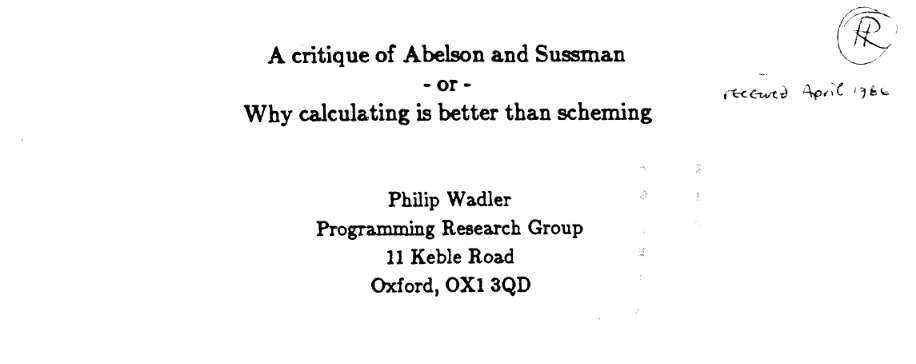
\includegraphics[scale=0.5]{wadler-title.png}
\end{frame}


\begin{frame}
\centering
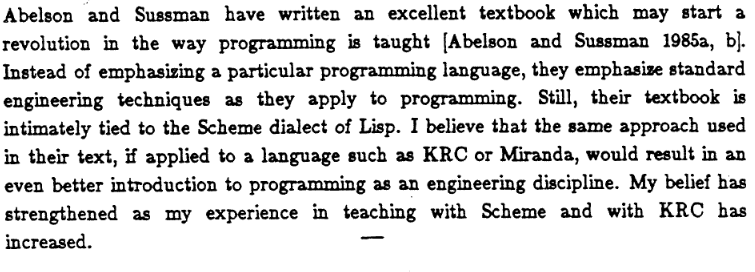
\includegraphics[scale=0.55]{wadler-abstract.png}
% TODO highlight bits?
\end{frame}

\begin{frame}[fragile]
\begin{haskellcode}
perimeter shape = case shape of
  Square s      -> s * 4
  Rectangle w h -> 2*w + 2*h
  Circle r      -> 2 * pi * r
\end{haskellcode}
\end{frame}


\begin{frame}[fragile]
\begin{schemecode}
(define (sum items)
  (cond ((null? items) 0)
        (else (+ (car items) (sum (cdr items))))))
\end{schemecode}

\pnl

\begin{haskellcode}
sum items = case items of
  []   -> 0
  x:xs -> x + sum xs
\end{haskellcode}
\end{frame}


\begin{frame}[fragile]
\begin{haskellcode}
[] ++ ys      =  ys
(x:xs) ++ ys  =  x:(xs ++ ys)
\end{haskellcode}

\begin{haskellcode}
(xs ++ ys) ++ zs = xs ++ (ys ++ zs)
\end{haskellcode}
\end{frame}

\iffalse
\begin{frame}[fragile]
\begin{schemecode}
(define (map proc items)
  (if (null? items)
      nil
      (cons (proc (car items))
            (map proc (cdr items)))))
\end{schemecode}
\nl

\begin{haskellcode}
map :: (a -> b) -> [a] -> [b]
map f l =
  case l of
    []       -> []
    (x : xs) -> f x : map f xs
\end{haskellcode}
\end{frame}


\begin{frame}[fragile]
\LARGE
\begin{schemecode}
             (list 3 4)

             (cons 3 4)
\end{schemecode}
\end{frame}


\begin{frame}[fragile]
\begin{columns}[T]
\LARGE
\column{0.5\textwidth}
\begin{schemecode}
  (cons 3 4)
\end{schemecode}

\includegraphics{list-cons1.pdf}

\column{0.5\textwidth}
\begin{schemecode}
  (list 3 4)
\end{schemecode}
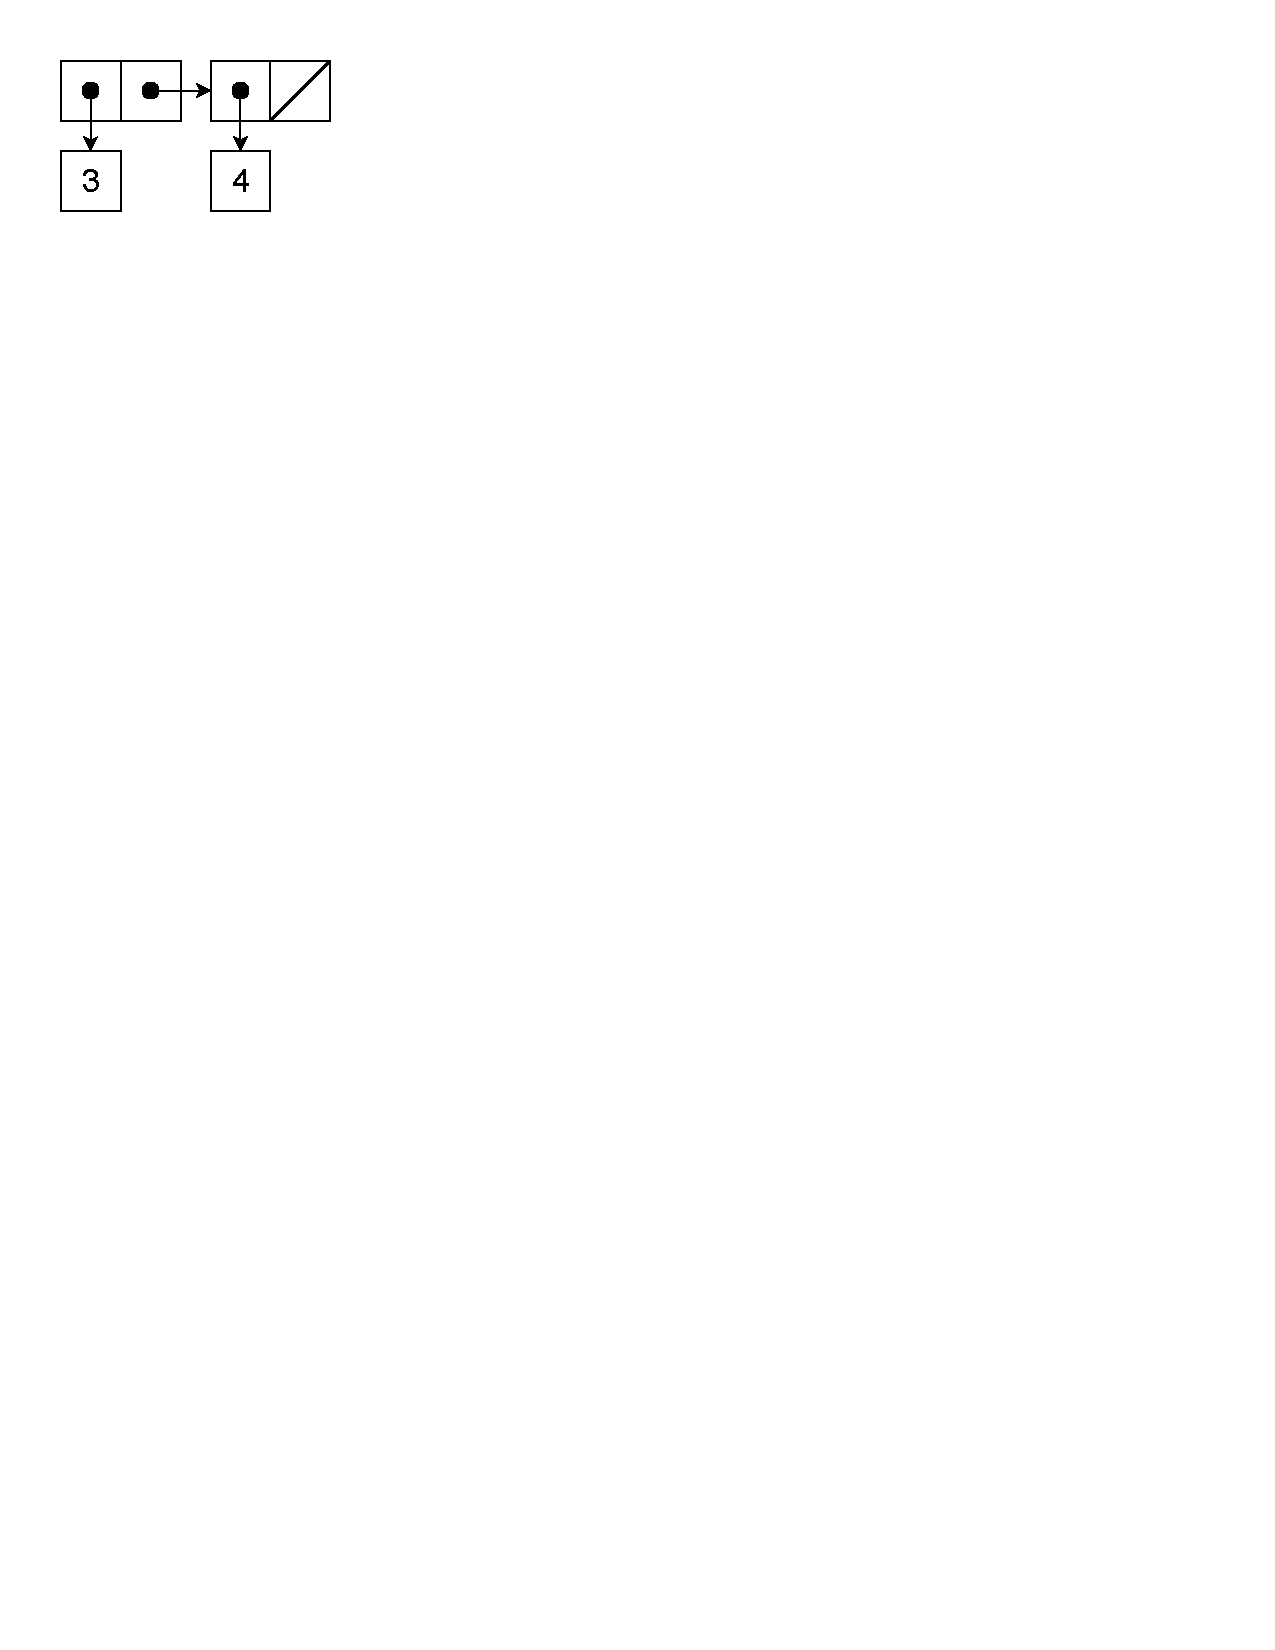
\includegraphics{list-cons2.pdf}
\end{columns}
\end{frame}


\imageslide[0.7]{list-cons-racket.png}
\fi


\imageslide[1.3]{pushout1.pdf}
\imageslide[1.3]{pushout2.pdf}


% TODO Haskell For Mac screenshot


\begin{frame}[fragile]

\Large
\begin{texttt}
3 + False
\end{texttt}
\nl

\large
\begin{block}{}
\begin{Verbatim}
<interactive>:1:1: error:
    • No instance for (Num Bool) arising from a use of ‘+’
    • In the expression: 3 + False
      In an equation for ‘it’: it = 3 + False
\end{Verbatim}
\end{block}
\end{frame}


\begin{frame}[fragile]

\begin{block}{Prelude.hs}
\begin{haskellcode}
module Prelude
  ( N.Integer, (+)
  , (==), Bool (..)
  )
where

import Data.Bool (Bool (..))
import qualified Data.Eq as E
import GHC.Num (Integer)
import qualified GHC.Num as N

(+) :: Integer -> Integer -> Integer
(+) = (N.+)

(==) :: Integer -> Integer -> Bool
(==) = (E.==)
\end{haskellcode}
\end{block}
\end{frame}


% TODO talk about custom type error machinery


% TODO Helium?


\begin{frame}
\huge \centering
Thanks for listening!
\end{frame}


%\begin{frame}
%\frametitle{Attributions}
%\begin{itemize}
%\item
%  Structure and Interpretation of Computer Programs \\
%  Harold Abelson and Gerald Jay Sussman with Julie Sussman \\
%  Attribution-ShareAlike 4.0 International (CC BY-SA 4.0)
%\item
%  How to Design Programs \\
%  Matthias Felleisen, Robert Bruce Findler, Matthew Flatt, Shriram Krishnamurthi \\
%  Attribution-NonCommercial-NoDerivs 2.0 Generic (CC BY-NC-ND 2.0)
%\end{itemize}
%\end{frame}


\end{document}

